
\chapter{Introduction}

% First paragraph has no indentation.

\noindent Many researchers believe the computer has become the third
method to do research, behind theory and experimentation, for both
science and engineering. Although there is no complete agreement on
the position intended for scientific computing with respect to the
other two methods, it is undeniable that computational methods are
an essential tool in most disciplines, particularly in those related
to decision making.

Nowadays, decision making is present practially everywhere. As scientistis,
engineers and managers have to make decisions in more complex and
competitive circumnstances every day, decision making involves dealing
with rational and optimal approaches. According to Talbi \cite{Talbi_Metaheuristics:2009},
decision making consists in the following steps:
\begin{itemize}
\item formulate the problem,
\item model the problem, 
\item optimize the problem, and
\item implement a solution.
\end{itemize}
Formulating a decision problem means making an initial statement about
it. Despite this first formulation may be imprecise, the objectives
of the problem are outlined, together with internal and external factors
that have some degree of influence over it. During the modelling of
the problem, an abstract mathematical model is built for it. Sometimes
this model is inspired by similar models in the literature, making
it possible to tackle the problem with well-studied methods. After
a model of the problem is available, the optimization step, i.e. generating
``good'' solutions for the problem, may begin. It is worth pointing
out that the resulting solutions are given for the abstract model,
and not for the original problem itself. Therefore, the performance
of the obtained solution is indicative when the model is an accurate
one \cite{Talbi_Metaheuristics:2009}. In the last step, the obtained
solution is practically tested by the decision maker and implemented
if it is an ``acceptable'' or ``good'' one. In case of ``bad''
or ``unacceptable'' solutions, the decision-making process is repeated,
possibly improving the model and/or the optimization algorithm. The
process, as described here, is depicted in Figure \ref{fig:01-decision_making_process}.

\begin{figure}
\centering

\includegraphics[width=0.4\textwidth]{02-background_and_motivation/img/optimization_cycle}

\caption{The classical decision-making process, as presented in \cite{Talbi_Metaheuristics:2009}.
Multiple iterations of this process improve the optimization algorithm
and/or model until an acceptable solution is found. \label{fig:01-decision_making_process}}
\end{figure}


\bigskip{}


Scientific computing, by means of computer-science methodology, makes
possible the study of problems that are too complex to be treated
analytically, or those that are very expensive or dangerous to be
studied by direct experimentation. Real-world problems are typically
very complex systems to be directly assessed by analytical models,
and require a numerical simulation for their study. Computer simulations
provide a resource to mimic the behavior of complex systems, by numerically
evaluating a model and gathering its data to estimate their true characteristics
\cite{law2007simulation}.

A model is a simplified representation of a studied problem, and one
of its purposes is to predict the effects of variations within the
system. A good model is a balance between realism and simplicity.
The system simulation, on the other hand, is the operation of the
model. Its configuration can also be changed, allowing multiple experimental
executions, something that might not be possible with the real system
it represents \cite{maria1997introduction}. However, it is important
to understand that the models used in scientific simulations and engineering
never offer a perfect model of the system they represent, but only
a subset of its composition and dynamics. For this reason, experimentation
and expert observation will always be essential as reference points
for understanding the studied phenomena. Consequently, problems categorized
as of large size and of considerable complexity represent a challenge,
because of the different involved disciplines and the degree of difficulty
of their modeling. Radio networks, in particular those of the third
and fourth generations, fall under this characterization.

Radio networks represent one of the most fast-growing technology markets
since the introduction of the Global System for Mobile communications
(GSM\nomenclature[A]{GSM}{Global System for Mobile communications.})
\cite{3GPP_TR_50.099} as the second generation (2G\nomenclature[A]{2G}{Second Generation of mobile networks.})
mobile networks more than twenty years ago. Its successor, the Universal
Mobile Telecommunications System (UMTS\nomenclature[A]{UMTS}{Universal Mobitel Telecommunications System.})
\cite{3GPP_TR_23.101} marks an evolution from 2G, representing a
milestone for the third generation of mobile radio networks (3G).
In recent years, the first commercial networks implementing the Long
Term Evolution (LTE), also known as fourth generation (4G) LTE, have
also appeared {[}ref???{]}. The always increasing demand for more
bandwidth has been one of the main forces behind the standardization
and later implementation of systems delivering higher speed data services
in order to improve the user's experience.

This evolution, first from 2G to 3G and later from 3G to 4G, has introduced
not only the technology needed to increase both data-transfer capacity
and voice quality, but also a greater complexity in terms of radio-network
planning, deployment, and configuration. This fact has attracted the
attention of the research community into areas such as the design
and optimization of radio-networks.

In a traditional or manual approach, during the design phase of a
radio network, a software tool would execute the analysis, while the
human would make the change decisions. Therefore, a radio engineer
configures the network parameters manually and the software tool analyzes
the given configuration. If the obtained results are not acceptable,
the analysis process has to be repeated several times, until the goal
is achieved. We will refer to this process as manual radio-network
optimization. 

Advances in the last few years have improved the manual optimization
process by introducing different problem-solving approaches that increase
the role the computer has during the optimization of radio networks,
consequently enlarging the scope of problems and instance sizes that
may be subject to automated optimization. Still, there are some important
aspects that restrict the utilization of these methods not only in
real-world enviroments, but also when doing research in the area of
optimization of radio networks:
\begin{itemize}
\item It is usually the case that the selected method is a compromise between
solution quality and computational-time complexity. The proposed state-of-the-art
approach for the evaluation of radio networks is the Monte-Carlo snapshot
analysis. However, real-world environments, where radio-network design
is carried out, require the evaluation of networks comprising up to
thousands of base stations in a reasonable amount of time. Moreover,
for applications involving radio-network optimization, multiple thousand
evaluations are required to find a good solution, in which case also
snapshot simulations are too time-consuming to be employed. Therefore,
for such applications and environments, methods with improved time
efficiency are required.
\item A considerable number of publications in the field of radio-network
optimization, of which we cite just a few for reference purposes \cite{amaldi2007radio_planning,siomina2007minimum_pilot_power,chen2008automated,chen2009fast,gordejuela2009two,siomina2008enhancing},
base their simulations on platforms for which it is not possible to
reproduce the experiments, either because they have used proprietary
software or because the data is not available. This fact reduces the
possibilities for comparing different approaches among each other,
and significantly contrasts with other research areas, such as evolutionary
computing or artificial intellingence, which have a set of open and
well-known benchmarks for the community to use. Thus, an open and
standardized framework would allow researchers to compare different
methods and results in a simple and objective manner.
\item Available commercial tools for radio-network evaluation have major
drawbacks with respect to the size of networks that can be considered,
simulation time, and especially the accuracy of the modeled system.
Yet, if precise and fast methods were commercially available, the
would lack the level of flexibility required by the scientific community.
Consequently, an essential attribute of the framework is to be open
source, so that anyone could extend it to meet some specific requirements.
In the long term, this process should also extend the set of built-in
functionality.
\item Particularly for path-loss predictions, created with empirical mathematical
models, the inaccuracy of the input data directly deteriorates the
precision of the calculated results. Moreover, since the physical
properties that influence the propagation of radio signals are not
constant and every environment introduces its own deviations, the
calculated coverage may be considered as not more than an approximation.
Therefore, there is a need for a method to adapt state-of-the-art
mathematical models for radio propagations so that the calculated
path-loss predictions are as accurate as possible, despite the various
sources of error noted before.
\end{itemize}
This thesis focuses on providing methods and tools to ??? the pointed
drawbacks. Short summary of the introduced novelties??? It is important
to note that some methods proposed in this thesis have been particularly
designed for problems emerging in radio planning of 3G networks. Despite
this, they may be adapted to other standards, e.g. GSM or LTE, without
lose of generality.


\section{Scope}

In this thesis, we intend to contribute methods and tools that will
provide solutions to the disadvantages pointed out in the previous
section. The introduced methods and tools have a close correlation
with the simulation and optimization of radio networks, especially
those of the 3G and 4G. We will introduce the steps necessary to mitigate
the problem of experimental reproducibility found in most published
works, by simplifying setup, execution, and sharing of experimental
results. With the development of the framework, we will evaluate and
assess the possibilities it offers as a support system for simulation
and optimization problems of radio networks. By including parallel
programming techniques for computer clusters and GPUs, we intend to
go beyond the classical methodology provided by previous works, taking
advantage of the inherent parallelism of some optimization techniques.
We will also be looking into the application of many advances in HPC
that should provide the framework with the computing power needed
to improve the simulation process, thus enhancing its scalability
to support real-world 3G radio networks. Finally, since we believe
that this work will only become truly productive through the cooperation
and long-term development of the scientific and engineering community,
we will be releasing the source code, algorithms, documentation, and
data to the public domain. This way, anyone will be able to use and
to extend the framework for their own needs. Encouraging cooperation
and sharing of experimentation-related tools and data should be a
common goal from which everyone will benefit.


\section{Hypothesis and aims}
\begin{itemize}
\item The great proportion of published works about optimization problems
for 3G radio networks is very difficult to reproduce, if possible
at all.
\item A common and open framework, designed for simulation of 3G radio networks,
should mitigate the experimental reproducibility problem by simplifying
sharing of experimental results.
\item Parallelization techniques improve the scalability and time requirement
of the framework, thus making it possible to process real-world data
sets.
\item Using hardware, specialized for parallel execution (e.g. GPU), improves
the time requirement of parallel algorithms using threads or message-passing
mechanisms.
\end{itemize}
Aims
\begin{itemize}
\item Analyze the state-of-the-art of optimization problems for 3G radio
networks in general, and UMTS in particular.
\item Identify common obstacles in optimization problems for 3G radio networks
that prevent them from being reproducible by other members of the
research community.
\item Design and implement framework tools to provide a common open environment
that will enable the scientific community to easily share and reproduce
different experimental conditions for maintenance and optimization
of 3G radio networks.
\item Integrate parallelization techniques to provide framework scalability,
so that it will be able to deal with large real-world data sets.
\item Evaluate the framework design by reproducing optimization environments
and introducing new algorithms for tackling previously unsolved instances
of optimization problems in 3G radio networks.
\item Evaluate and analyze all experimental results and simulations in the
context of real networks, using real-world data.
\end{itemize}

\section{Methodology}

The dissertation will use the following methodology to prove the hypothesis
stated in the previous sections.

First, we will survey existing optimization problems and techniques
for 3G radio networks in general, and UMTS in particular. The focus
of the survey will be on optimization problems that do not provide
the means required by experimental reproducibility and require the
use of a snapshot-based model of the radio network.

Second, we will design and develop a parallel framework for radio
network simulations. The development of the framework will focus on
joining optimization and simulation, so that it will cover a wider
range of use cases, namely as a maintenance and optimization tool
for 3G radio networks. Additionally, we will make an intensive study
of the mathematical models currently used, seeking to assess their
reliability when used in simulations of 3G radio networks. Since the
algorithms and simulations used in the optimization of 3G radio networks
consume large amounts of data and require high computing power (due
to the large number of simulations they need to run), we will improve
the performance of the framework even more by adapting its most time-consuming
parts for execution on GPUs.

Finally, we will evaluate the benefits of the above-mentioned framework
by conducting reproducible experiments that will support the hypothesis
outlined under ???, by tackling similar and bigger problem instances
when solving both well-known and new optimization problems for 3G
radio networks.


\section{Contributions}

The expected contributions of this dissertation to the fields of telecommunications
and computer sciences include the following:
\begin{itemize}
\item State-of-the-art overview of optimization methods for 3G radio networks.
\item Design and development of a framework that provides an open environment
for radio network simulations, implemented for execution on computer
clusters and GPUs. The framework will allow the scientific community
to share a common domain to run the simulations needed by modern optimization
methods, since most currently available simulation tools are proprietary
and therefore unsuitable for experimental reproducibility.
\item Improvement of quality and speed of renowned mathematical models,
used for radio propagation predictions, by applying parameter optimization
and parallelization techniques. The expected speed improvement should
be of at least one order of magnitude.
\item Proposal of a new algorithm, based on autonomous agents, to solve
the service coverage problem. The solved problem instances should
be of bigger size than ever solved in the literature and reach equal
or better quality thereof. This should make our approach applicable
for large real-world problem instances and data sets.
\item Identification of a new optimization problem in 3G radio networks
that deals with soft-handover alignment of downlink and uplink areas.
By solving this problem, we should avoid abnormal network functioning
in areas where there is soft-handover capability in the uplink, but
none in the downlink. So far this problem has been solved manually
by radio experts.
\item Empirical comparison of the proposed metaheuristic algorithm against
the existing state-of-the-art optimization algorithms on the soft-handover
alignment problem.
\end{itemize}

\section{Organization}

The introduction provided in this chapter pretends to delimiter the
context within which the dissertation will address.

The rest if this dissertation is organized as follows.

Chapter \ref{chap:Background-and-motivation} present an overview
of some well-known optimization problems that occur during deployment
and configuration of mobile networks. A description of each optimization
problem is given, followed by a short survey of recently proposed
optimization methods. It closes by giving a conclusion regarding mobile
networks and why they are a rich source of optimization problems.

Chapter \ref{chap:Framework-parameter-tuning} deals with the automatic
tuning of parameters of the mathematical models, used for radio propagation
predictions. Namely, based on field measurements, the configurable
parameters of the mathematical models used by the framework may be
automatically tuned to minize the deviation from the prediction to
the actual state of the network.

In Chapter \ref{chap:Experimental-evaluation-the-SHO-alignment-problem},
a static network simulator is used to find downlink and uplink SHO
areas. By introducing a penalty-based objective function and some
hard constraints, we formally define the problem of balancing SHO
areas in UMTS networks. The state-of-the-art mathematical model used
and the penalty scores of the objective function are set according
to the configuration and layout of a real mobile network, deployed
in Slovenia by Telekom Slovenije, d.d.. The balancing problem is then
tackled by three optimization algorithms, each of them belonging to
a different category of metaheuristics. We report and analyze the
optimization results, as well as the performance of each of the optimization
algorithms used.

Chapter \ref{chap:Experimental-evaluation-the-service-coverage-problem}
considers the problem of minimizing the total amount of pilot power
subject to a full coverage constraint. Our optimization approach,
based on parallel autonomous agents, gives very good solutions to
the problem within an acceptable amount of time. The parallel implementation
takes full advantage of GPU hardware in order to achieve impressive
speed-up. We report the results of our experiments for three UMTS
networks of different sizes based on a real network currently deployed
in Slovenia.
